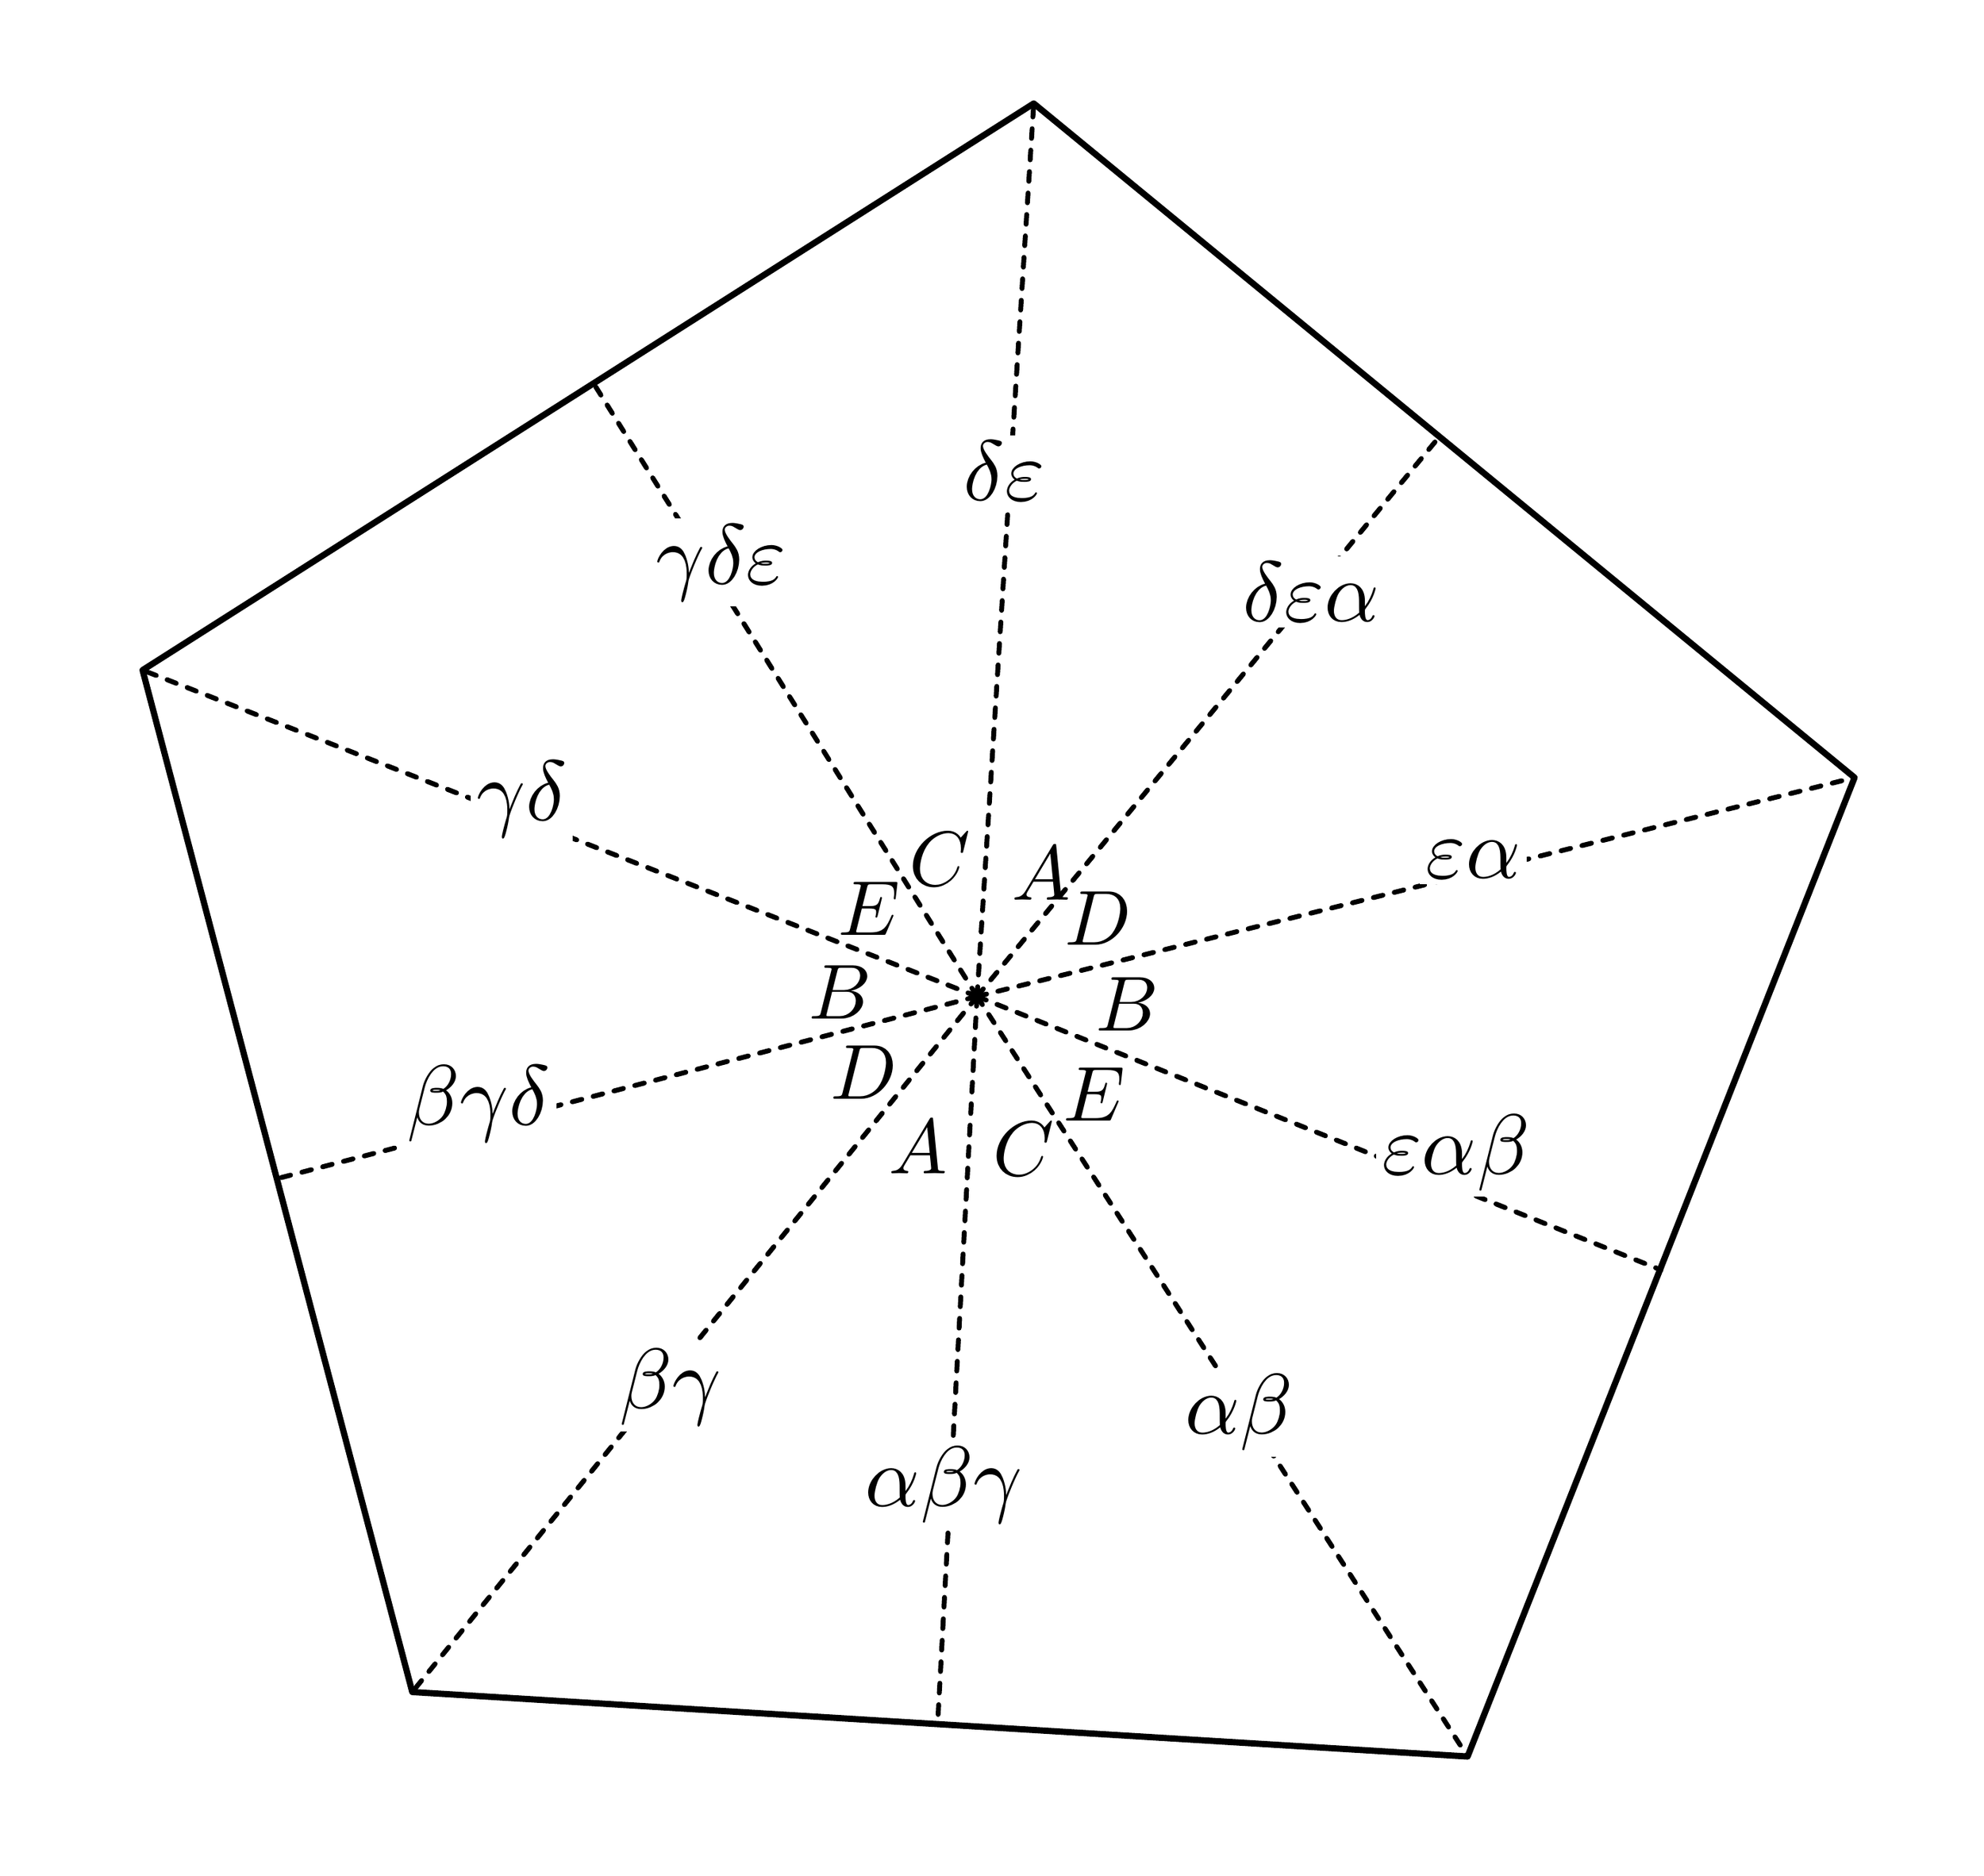
\begin{tikzpicture}[x=1bp,y=-1bp,line cap=round,line join=round]
\path[use as bounding box] (0,0) rectangle (995,940);
\begin{pgfinterruptboundingbox}
\draw[line width=3.2bp] (63,333) -- (519,43) -- (939,388) -- (741,889) -- (201,856) -- cycle;
\draw[line width=2.5bp,dash pattern=on 5bp off 6bp] (490,500) -- (293,185);
\draw[line width=2.5bp,dash pattern=on 5bp off 6bp] (490,500) -- (519,43);
\draw[line width=2.5bp,dash pattern=on 5bp off 6bp] (490,500) -- (727,213);
\draw[line width=2.5bp,dash pattern=on 5bp off 6bp] (490,500) -- (939,388);
\draw[line width=2.5bp,dash pattern=on 5bp off 6bp] (490,500) -- (840,640);
\draw[line width=2.5bp,dash pattern=on 5bp off 6bp] (490,500) -- (741,889);
\draw[line width=2.5bp,dash pattern=on 5bp off 6bp] (490,500) -- (470,869);
\draw[line width=2.5bp,dash pattern=on 5bp off 6bp] (490,500) -- (201,856);
\draw[line width=2.5bp,dash pattern=on 5bp off 6bp] (490,500) -- (129,594);
\draw[line width=2.5bp,dash pattern=on 5bp off 6bp] (490,500) -- (63,333);
\node[fill=white,inner sep=3bp,outer sep=0pt,rotate=0] at (504,231) {\scalebox{4.4}{\ensuremath{\delta\varepsilon}}};
\node[fill=white,inner sep=3bp,outer sep=0pt,rotate=0] at (661,293) {\scalebox{4.4}{\ensuremath{\delta\varepsilon\alpha}}};
\node[fill=white,inner sep=3bp,outer sep=0pt,rotate=0] at (744,430) {\scalebox{4.4}{\ensuremath{\varepsilon\alpha}}};
\node[fill=white,inner sep=3bp,outer sep=0pt,rotate=0] at (735,580) {\scalebox{4.4}{\ensuremath{\varepsilon\alpha\beta}}};
\node[fill=white,inner sep=3bp,outer sep=0pt,rotate=0] at (624,713) {\scalebox{4.4}{\ensuremath{\alpha\beta}}};
\node[fill=white,inner sep=3bp,outer sep=0pt,rotate=0] at (473,750) {\scalebox{4.4}{\ensuremath{\alpha\beta\gamma}}};
\node[fill=white,inner sep=3bp,outer sep=0pt,rotate=0] at (333,700) {\scalebox{4.4}{\ensuremath{\beta\gamma}}};
\node[fill=white,inner sep=3bp,outer sep=0pt,rotate=0] at (235,555) {\scalebox{4.4}{\ensuremath{\beta\gamma\delta}}};
\node[fill=white,inner sep=3bp,outer sep=0pt,rotate=0] at (257,399) {\scalebox{4.4}{\ensuremath{\gamma\delta}}};
\node[fill=white,inner sep=3bp,outer sep=0pt,rotate=0] at (359,278) {\scalebox{4.4}{\ensuremath{\gamma\delta\varepsilon}}};
\node[inner sep=0pt,outer sep=0pt,rotate=0] at (471,430) {\scalebox{4.0}{\ensuremath{C}}};
\node[inner sep=0pt,outer sep=0pt,rotate=0] at (523,437) {\scalebox{4.0}{\ensuremath{A}}};
\node[inner sep=0pt,outer sep=0pt,rotate=0] at (552,460) {\scalebox{4.0}{\ensuremath{D}}};
\node[inner sep=0pt,outer sep=0pt,rotate=0] at (567,504) {\scalebox{4.0}{\ensuremath{B}}};
\node[inner sep=0pt,outer sep=0pt,rotate=0] at (550,550) {\scalebox{4.0}{\ensuremath{E}}};
\node[inner sep=0pt,outer sep=0pt,rotate=0] at (514,578) {\scalebox{4.0}{\ensuremath{C}}};
\node[inner sep=0pt,outer sep=0pt,rotate=0] at (460,577) {\scalebox{4.0}{\ensuremath{A}}};
\node[inner sep=0pt,outer sep=0pt,rotate=0] at (432,539) {\scalebox{4.0}{\ensuremath{D}}};
\node[inner sep=0pt,outer sep=0pt,rotate=0] at (420,498) {\scalebox{4.0}{\ensuremath{B}}};
\node[inner sep=0pt,outer sep=0pt,rotate=0] at (435,455) {\scalebox{4.0}{\ensuremath{E}}};
\end{pgfinterruptboundingbox}
\end{tikzpicture}
